\documentclass[12pt]{article}
\usepackage{amsmath}
\usepackage{amsfonts}
\usepackage{graphicx}
\DeclareGraphicsExtensions{.pdf,.png,.jpg}
\usepackage{algpseudocode} 

\newtheorem{theorem}{Theorem}[section]
\newtheorem{lemma}[theorem]{Lemma}
\newtheorem{definition}[theorem]{Definition}


\title{Reducing Small Discs}
\date{}
\begin{document}
  \maketitle
  
  \section{Demo}
  Graph below shows covering left areas by sampling iso-cost discs. 
  
  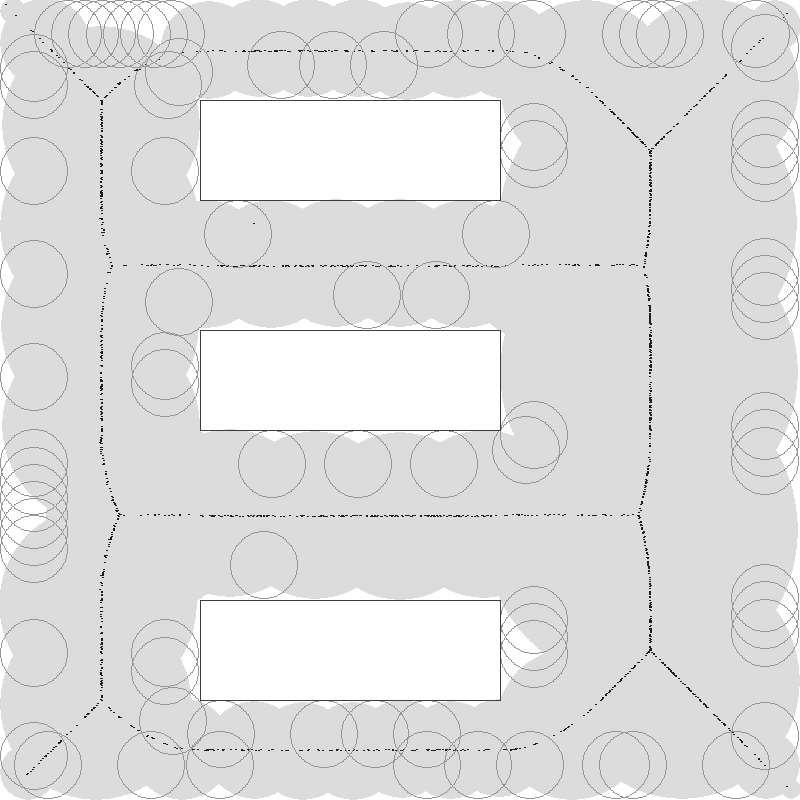
\includegraphics[scale=0.5]{MedialAxis_bnd_iso_better.PNG}  
  
  \section{Algorithm}

	\subsection{Measuring newly discovered area}
    Say we have a disc $ball(O_1, R)$ already, and a new disc $ball(O_2, r)$. The newly discovered area, read shaded in the graph, can be expressed as a function of $x$, denoted as $f(x)$. Obviously, $f(x)$ is monotonically increasing when $x \in [0, 2\cdot r]$. We can measure if a new disc discovers enough new area by measuring if $x$ is larger than a threashold. ( $x = d+r-R \geq threashold$ )
    
    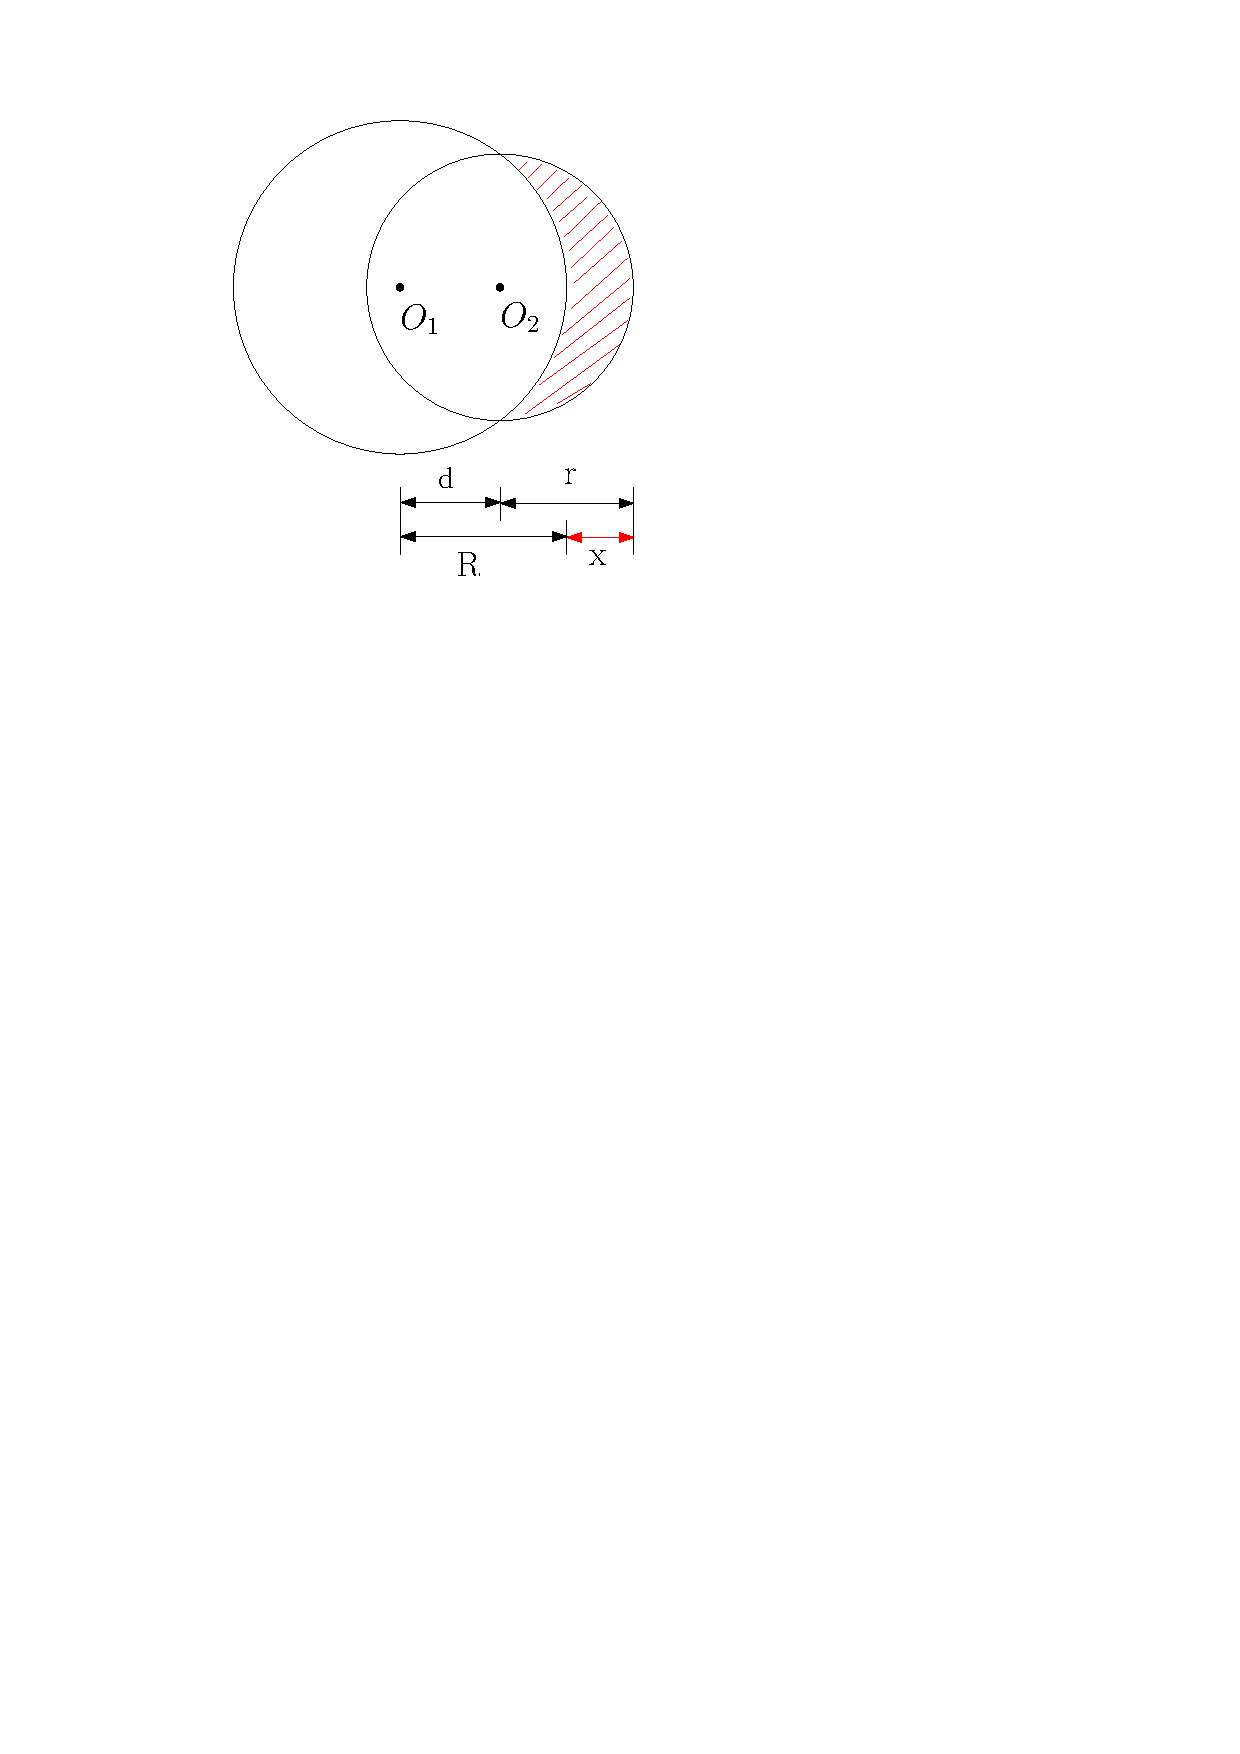
\includegraphics[scale=1]{measuring_new_cover.pdf}
	
    Although this $f(x)$ function determines the relation between one new disc and another existing disc instead of a set of existing discs. The result seems pretty good. (No idea why, yet.)\\
	
	
	Measuring if a disc is useful:\\  
  
	\begin{algorithmic}
    \State $maSamples \gets$ medial axis samples.	
	\State $isoSamp \gets$ one iso-cost sample. 
	\For{$samp \in maSamples$}
		\State $centerdist \gets |samp.center - isoSamp|$  \Comment{Distance between centers}
		\If{ $centerdist + isoSamp.radius - samp.radius \leq threashold$ }
			\indent \indent \Return False 
		\EndIf
	\EndFor
	
	\noindent \Return True;
	\end{algorithmic}
	
	
	\subsection{Generating small discs to cover left areas}
	
	\begin{enumerate}
	\item Generate Medial Axis Samples.
	\item Generate iso-cost small discs. Every disc is some distance away from existing ones.
	\item Test every iso-cost disc to see if it is useful. Keep only useful ones.
	\end{enumerate}
	
	\section{Questions}
		
	\begin{enumerate}
	\item Why the method to measure new discovered area works.
	\item How densely should we sample iso-cost discs?
	\item Which size disc should we sample?
	\end{enumerate}
	
  
\end{document}